% Chapter 1

\chapter{Introduction} % Main chapter title

\label{Chapter1} % For referencing the chapter elsewhere, use \ref{Chapter1} 

%----------------------------------------------------------------------------------------

% Define some commands to keep the formatting separated from the content 
\newcommand{\keyword}[1]{\textbf{#1}}
\newcommand{\tabhead}[1]{\textbf{#1}}
\newcommand{\code}[1]{\texttt{#1}}
\newcommand{\file}[1]{\texttt{\bfseries#1}}
\newcommand{\option}[1]{\texttt{\itshape#1}}

%----------------------------------------------------------------------------------------

\section{Background}

\setlength{\parindent}{10ex} Nearly three and half centuries passed since Antony Van Leeuwenhoek had drawn a benchmark for biological imaging by discovering “little animals ”, present day microbes, using his microscopes. His breakthrough paved a road to scientists and biologists to study tinny structures of living things. At that time, Leeuwenhoek’s main curiously was to magnify his “little animals”, protozoa and bacteria, and then study their structure though he was the first one to see and describe sperm and blood cells \cite{Croft2006,Dobell1960}. Since then, scientists and technologists have devoted and carried out remarkable works to magnify and study micro (small) level events and macro (large) level hidden or distant objects or structures. Micro level imaging technologies such as Scanning Probe Microscope (SPM), Transmission Electron Microscope (TEM) and Scanning Electron Microscope (SEM) help scientists and researchers to study immensely smaller resolution structures or objects \cite{Croft2006}.On the other hand, macro level imaging technologies such as X-ray, CT, MRI, PET, Ultrasound and SPECT help the physicians and researchers to understand anatomy and physiology of normal and abnormal internal hidden organs/tissues of human being \cite {Dhawan2011}. As well, macro level imaging technologies such as astrological telescopes help cosmologists to see distant cosmic objects \cite{Russ2016}.

The revolution of digital and information technology after the second half of the 20th century dominates the traditional analog way of imaging and simplify the method how images are acquired (both in time and process), processed, stored, displayed and transmitted from one place to the other. For example, these days, most molecular and cellular study laboratory microscopes have been integrated with high frame rate cameras. These high speed cameras will help the researcher to capture the photographs of cellular or molecular micron activities that are happened with in a fraction of second and store them for off-line studies.

The main purpose of this thesis work is to segment red blood cells of near to endothelial lining that are disturbed by ultrasonic energy and make them suitable for studying their micro activities.  The next subsection mainly focuses on image segmentation concepts such as types, commonly known techniques and challenges. Subsequently, discussions on preliminary concepts related to red blood cells, ultrasonic energy and microscale events of red blood cells near to endothelial lining will be presented. 

\begin{figure}[th]
	\centering
	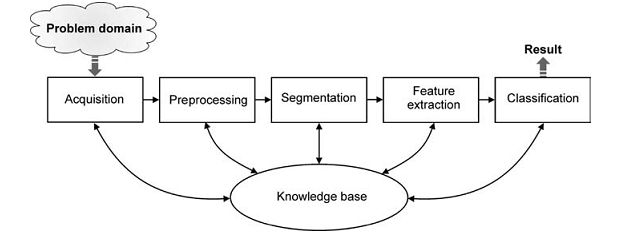
\includegraphics{Figures/computervisionsystem.png}
	%\decoRule
	\caption[Computer Vision System]{Computer vision system.}
	\label{fig:Computer Vision System}
\end{figure}


%----------------------------------------------------------------------------------------

\section{Statement of Problem}

Experimental results from previous work (Mazzawi et al., 2015) showed that sonication of mixture of blood, polystyrene microspheres and ultrasound contrast agent forces particles and cells  to migrate towards the nodes of the sound field. Particles and cells create a circular pattern as shown on Figure 5. When the sonication filed is halted the particles/cells trapped at the nodes remain there and the rest wobble inside the ring. All blood cells, ultrasound contrast agent and polystyrene microspheres are responsible for the circular pattern formation. However, ultrasound contrast agent microbubbles behave differently. They accumulate in circles at the nodes faster than blood cells and polystyrene microspheres and create a strong clusters as illustrated on Figure 6 which is not possible in blood cells and polystyrene particles due to weak Bjerknes forces. Besides, sonophore model of cells doesn’t allow strong cluster formation.
\begin{figure}[th]
	\centering
	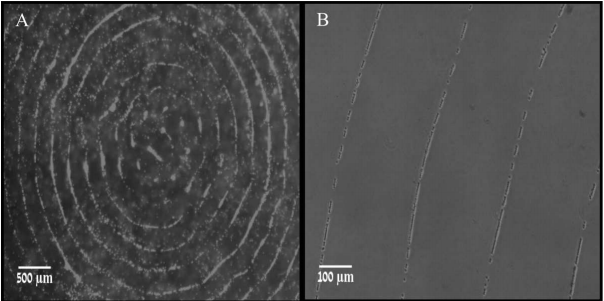
\includegraphics{Figures/CircularPattern.png}
	%\decoRule
	\caption[Circular Pattern Formation of Cells]{Ultrasound contrast agent (Quantison microbubbles) accumulated in circles(left) and form tightly packed cluster(right)}
	\label{fig:Circular Pattern Formation of Particles}
\end{figure}


\bibliographystyle{plain}
\bibliography{SelectedReferences/MScThesisChapterI}